\chapter{Mejoras estructurales}
	
	\section{Desenfoque: Modelo de lente fina}
	
	Hasta ahora se ha estado utilizando un modelo de cámara ideal denominado cámara estenopeica. Esta cámara tiene la particularidad de tener un enfoque perfecto siempre, siendo una propiedad indeseada en un motor de renderizado fotorrealista, ya que la mayoría de las cámaras reales incluyen lentes en su estructura que desvían los rayos de luz gracias a la difracción del cristal, enfocando a determinada distancia, y desenfocando el resto de la escena. El hecho de poder enfocar a una distancia determinada permite hacer énfasis en un sujeto de la escena, y desenfocar el resto. Este efecto se conoce como ``Bokeh`` y es muy deseado en un motor de renderizado, puesto que es un recurso cinematográfico muy atractivo visualmente.

	Para solventar el problema del enfoque perfecto se va a hacer uso de un modelo de cámara denominado modelo de lente fina. Este modelo es una simplificación de lo que sería una simulación física de unas lentes reales. Al simplificar los cálculos, se pierden artefactos y desperfectos deseados como la aberración cromática o la distorsión de lentes, pero a cambio se obtiene la simplicidad de implementación.

	Para activar este efecto, es necesario compilar con la constante \code{BOKEH} definida. Esto desbloqueará la parte de código que hace el cálculo del desenfoque. 
	
	Este nuevo método añade a la clase \code{Camera} dos nuevas variables, por un lado \code{focusDistance} y por otro lado \code{aperture}. La primera define la distancia a la que se encuentra el plano de enfoque, y la segunda, la apertura en f-stops del iris de la cámara. 

	El procedimiento para calcular los rayos emitidos por el nuevo modelo de cámara es el siguiente:

	1: Se calcula el rayo original del método anterior, desde la cámara hasta el sensor.
	
	2: Se calcula la intersección de dicho rayo con el plano de enfoque, situado a la distancia \code{focusDistance}. La intersección se denomina \code{focusPoint}.
	
	3: En vez de emitir e rayo desde el punto de la cámara, se elige un punto aleatorio en el iris \code{iRP} y se emite un rayo desde ahí hasta el punto de enfoque \code{focusPoint}. Este nuevo rayo será un rayo bajo el modelo de cámara de lente fina. Los elementos situados a la distancia de enfoque \code{focusDistance} serán más nítidos que aquellos que no lo estén.

	\begin{figure}
		\centering
		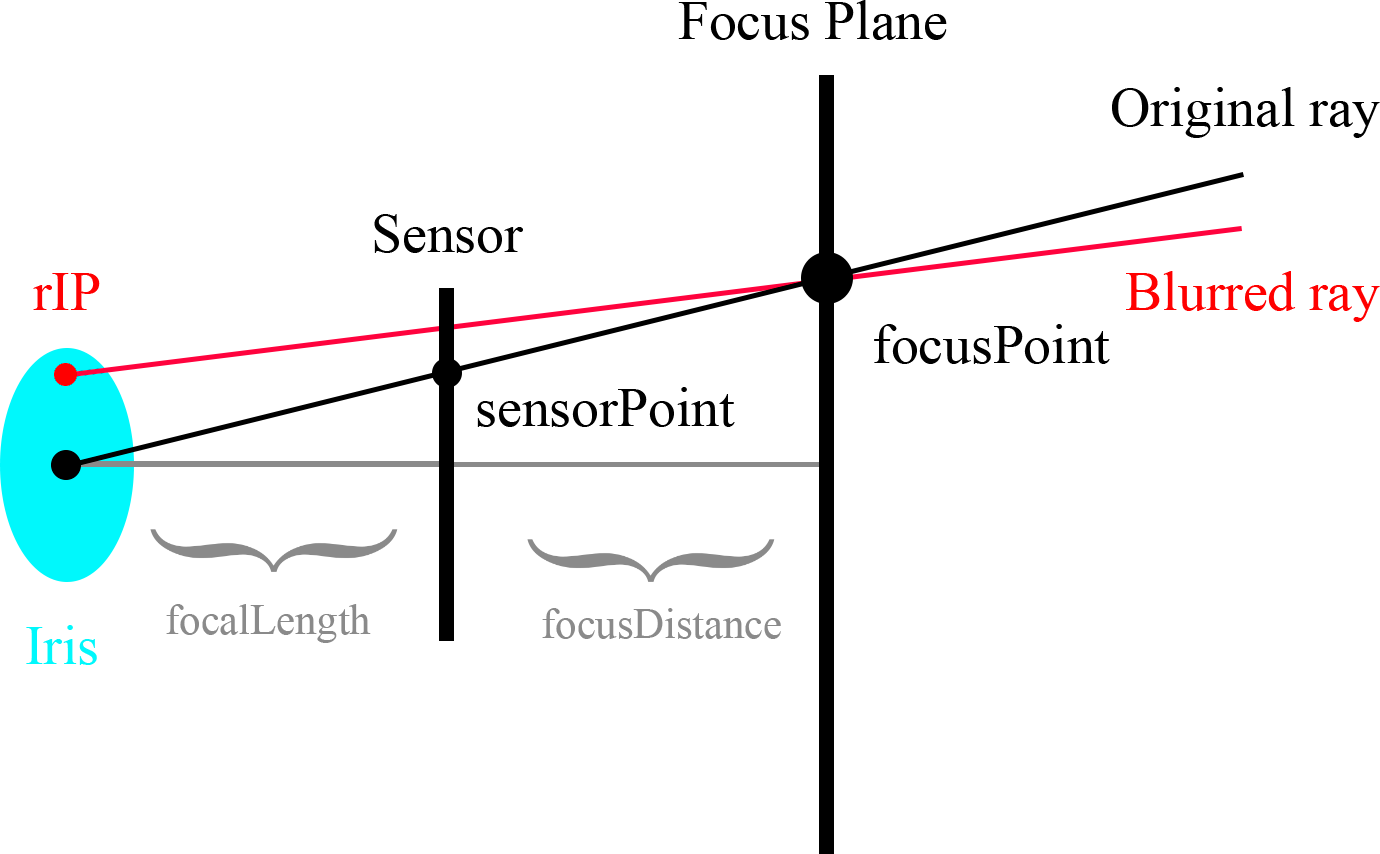
\includegraphics[width=0.5\textwidth]{blurring}
		\caption{}
		\label{fig:label}
	\end{figure}


	
	\section{Iluminación}
	
	La iluminación se define en este contexto como cualquier cuerpo capaz de emitir energía lumínica a la escena. Esta energía lumínica será multiplicada por el factor de reducción de cada fotón, determinado en cada rebote, y, añadida de manera lineal a la energía total del fotón.

	Luces de punto:

	Las luces de punto son quizá el elemento más simple de iluminación. Consisten en un punto sin volumen el cual emite radiación lumínica de manera uniforme. Esta radiación se desvanece de manera cuadrática. Debido a que son puntos infinitesimalmente pequeños, jamás serán alcanzados por los fotones emitidos desde la cámara, de manera que requieren un procesamiento especial explicado en el capítulo de Muestreo por importancia de luces de punto.

	Una luz de punto viene definida por tres atributos: Color, intensidad y posición. La energía lumínica viene dada por la ecuación:
	
	Materiales emisivos:

	Cuando un objeto es alcanzado por un rayo, lo más común es que se reste energía a dicho rayo debido a la absorción del material. Otra opción es sumarle energía. Si esto ocurre, se pasará a considerar a ese objeto como otra fuente de luz más.

	La energía sumada a dicho rayo será obtenida de una textura denominada emisión del material a través del mapeo correspondiente del punto de intersección, multiplicada así por un factor de intensidad.

	IBL (Image Based Lightning):

	La iluminación basada en imagen ha sido uno de los elementos más relevantes en las técnicas para el renderizado fotorrealista. Se utiliza ampliamente en la industria cinematográfica debido a la complejidad visual que aporta a una escena 3D y debido a que permite captar la iluminación de entornos reales y posteriormente añadirla en escenas digitales. El hecho de poder trasladar la iluminación a un escenario virtual, facilita la composición de modelos tridimensionales en películas y series de televisión donde es necesario juntar una grabación real con un elemento generado por ordenador.

	Esta técnica se basa principalmente en usar una fotografía de 360 grados como fuentes de luz formando una esfera alrededor de la escena. Estas fotografías son conocidas como HDRI (Imagen de Alto Rango Dinámico). A diferencia de las imágenes tradicionales las cuales normalmente tienen 8 bits de resolución por canal de color, las imágenes HDRI cuentan con valores de punto flotante. Esto es debido a que su uso no es meramente la visualización de estas en pantallas de 8 bits de resolución por color como la mayoría de imágenes, sino que el valor de cada píxel será utilizado para realizar las operaciones pertinentes para iluminar la escena.

	La implementación de esta técnica en el motor de render viene dada por el uso de una textura en formato .hdr (imágenes en punto flotante), o un color plano. En caso de utilizar una textura, se considerará cada píxel como una pequeña fuente de luz direccional en el infinito, orientada hacia el centro de la escena. 

	Los rayos que no interseccionan con nada se consideran que interseccionan en el infinito con el HDRI, por esta razón, al detectar que un rayo ha terminado de rebotar y ha terminado en el infinito, se obtendrá la dirección de este, y esta dirección se traducirá en las coordenadas polares del HDRI que posteriormente recuperarán el valor interpolado bilinearmente del pixel del HDRI correspondiente.


	\section{Texturas}
	
	Texturas:
	El uso de colores planos en los materiales limita la capacidad de imitación de la realidad. Un recurso esencial para romper esta limitación es el uso de texturas. Una textura consiste en una matriz bidimensional de valores en punto flotante.

	La implementación de las texturas viene dada en el código por la clase Texture.
	Coordenadas UV:

	Una vez se ha definido este tipo de coordenadas se pueden añadir parámetros que las modifiquen, estos parámetros se encuentran en la clase Texture.

	xTile e yTile: definen las veces que se repite una textura
	xOffset e yOffset: definen el desplazamiento de esta textura.
	Interpolado bilinear:
	El problema de las texturas es que cuentan con una resolución limitada. Esto provoca que se pixelice cuando se muestra cercana a la cámara. Una solución adoptada de manera general en muchos ámbitos es la interpolación los píxeles vecinos de manera lineal. 




	Por esta razón, cada vez que se quiera acceder a un píxel en las coordenadas UV, se devolverá el valor interpolado con la función getValueBilinear().

	
	\section{Sombreado BRDF}
	
		
	El sombreado consiste en dar un valor de pérdida de energía para un rayo que intersecciona con un punto. Así pues, en la industria es utilizada una función conocida como BRDF. Esta función define un valor para la radiación reflejada a partir de un ángulo entrante wi y un ángulo saliente wo.

	Un elemento clave del renderizado fotorrealista es elegir una función de sombreado apropiada. En este motor se ha hecho uso del modelo de sombreado Disney Principled Shader. Este modelo fue desarrollado por Disney bajo el fin de simplificar los parámetros de las fórmulas matemáticas y que estos sean cómodos para los artistas. Esta decisión tiene más sentido si consideramos el contexto histórico, donde los modelos anteriores contaban con parámetros complejos.

	Este modelo cuenta además con buen fotorrealismo, y por ello, el conocido software de edición 3d de código abierto Blender, hace uso de él como su modelo de sombreado primario.


	A continuación se muestra una lista con los parámetros de los materiales descritos bajo este modelo:

	roughness:
	metallic:
	clearcoatGloss:
	clearcoat:
	anisotropic:
	eta:
	specular:
	specularTint:
	sheenTint:
	subsurface:
	sheen:


	
	\section{Renderizado progresivo}
		
	Hoy en día, la mayoría de los motores de renderizado de producción son progresivos. Esto implica que las muestras se van acumulando poco a poco hasta que termina por converger la imagen deseada. Esto difiere de los motores de renderizado por CPU tradicionales, los cuales van procesando la imagen en recuadros de tamaño limitado. Se ha decidido hacer una implementación iterativa con el fin de estar más cerca del estado del arte.



	Este tipo de implementación se beneficia de la copia de datos asíncrona de la GPU. Mientras el kernel se ejecuta, un flujo de datos secundario hará la copia del buffer de la GPU en la CPU, pudiendo así actualizar la visualización del resultado varias veces por segundo.

	Este flujo de datos secundario se ha implementado con el tipo de datos ``cudaStream\_t`` de la API de CUDA. Han sido necesarios dos flujos, uno denominado ``kernelStream`` y otro denominado ``bufferStream``. Los kernels de inicialización y renderizado correrán en el primero, mientras que la función que obtiene el buffer, será lanzada en el segundo.
